% TODO: explain how depths are aligned to color images.
% TODO explain how tracking candidates are computed

\chapter{Derivations}
In this section we derive all necessary expressions that are required in order to implement our motion segmentation pipeline, which is described in the next chapter.

\section{Trajectory Affinities}
\label{sec:trajectory_affinities}
In this section we explain how we calculate similarities between extracted trajectories. This computation is the fundamental step of our work.
Before going into details, let us first revisit the definition of a trajectory. By the term trajectory we refer to a list of tracking points, which is ordered by the frame index in which each point was traced. Therefore, every points knows to which frame it belongs to. \\ \\
Let $A$, $B$ denote two trajectories resulting from the previous tracking step. Our goal is to define the similarity between the trajectories by computing a distance $d(A,B)$ between every trajectory pair. For that purpose we exploit their maximal dissimilarity via their maximal motion difference among all frames of common visibility. The squared version of this conceptual formula description is listed in equation $\ref{eq:prod_dist_affinity}$ 
\begin{equation}
	d^2 \left( A, B \right) = \max_t d_t^2 \left( A, B \right)
	\label{eq:product_distance}
\end{equation}
The resulting distance value from equation $\ref{eq:product_distance}$ is then turned into a affinity via the transformation
\begin{equation}
	w \left( A, B \right) = e^{ -\lambda d^2 (A, B) }.
	\label{eq:prod_dist_affinity}
\end{equation}
This measure is based on the work of Shepard $\cite{Shepard87}$ who proposed as a universal law that distance and perceived similarity are related via an exponential function.


where

\begin{equation}
	d_t^2 \left( A, B \right) = d_{spatial}^{A,B} \left( d_{motion}^{A,B} (t) \right) ^2
\end{equation}

\begin{equation}
	d_{spatial}^{A,B} = \frac{1}{\omega - \alpha + 1} \sum_{k=\alpha}^\omega \norm{A(k) - B(k)}
\label{eq:spatial_distance}	
\end{equation}
where $\alpha$ is the first- and $\omega$ is the last- overlapping frame index between the two given trajectories $A$ and $B$.

\begin{equation}
	d_{motion}^{A,B} \left( t \right)  = \frac{\norm{\partial_t A - \partial_t B}}{\sigma_t}
\label{eq:motion_distance}
\end{equation}
The expression $\partial_t A$ denotes the averaged motion over time, which is computed by approximating the derivatives $\partial_t A$, $\partial_t B$ using forward differences with a certain timestep $T$.

\begin{equation}
	\partial_t A = \frac{1}{T} \left( x_{t+T}^{A} - x_{t}^{A}, y_{t+T}^{A} - y_{t}^{A}\right)
\end{equation}
The exact value of $T$ is either the number of overlapping frames between the $A$ and $B$ or a fixed number, in case there are fewer common frames available, than a fixed threshold. \\ \\
Please note that by computing the affinity for every existing trajectory pair combinations, as defined in equation $\ref{eq:prod_dist_affinity}$, we implicitly encode a $n \times n$ affinity matrix $W$, for $n$ given trajectories. 

\section{Eigendecomposition of Graph Laplacians}
In this section we derive the Eigendecomposition of the graph Laplacian which will be used to implement a motion segmentation based on spectral clustering. The necessary theory can be looked up in section $\ref{sec:spectral_clustering_bg}$. \\ \\
Given the pairwise affinity matrix $W$ as computed in section $\ref{sec:trajectory_affinities}$ on page $\pageref{sec:trajectory_affinities}$. An example of such an matrix is shown in figure $\ref{fig:cars_affinity_mat_sub}$. An approximated partitioning of the underlying graph can be obtained by running a variant of spectral clustering. Let
\begin{equation}
	D = \text{diag} \left( d_{A_1}, \dots, d_{A_n} \right)
\label{eq:def_d_mat}
\end{equation}
be the $n \times n$ diagonal degree matrix with the entries
\begin{equation}
	d_{A_k} = \sum_B w \left( A_k, B \right)
\end{equation}
The eigendecomposition of the normalized graph Laplacian is given by equation $\ref{eq:normalized_graph_laplacian}$.
\begin{equation}
	V^{T} \Lambda V = D^{-\frac{1}{2}} \left( D - W \right) D^{-\frac{1}{2}}
	\label{eq:normalized_graph_laplacian}
\end{equation}
Where $V$ denotes a matrix containing the column-wise eigenvectors of the Laplacian and $\lambda$ is a diagonal matrix containing the corresponding eigenvalues. Figure $\ref{fig:cars_eigenvectors_laplacian}$ shows two example eigenvectors, resulting from the $\textit{cars}$ dataset.

\begin{figure}[H]
\begin{center}
\subfigure[Eigenvector Front-Car]{
   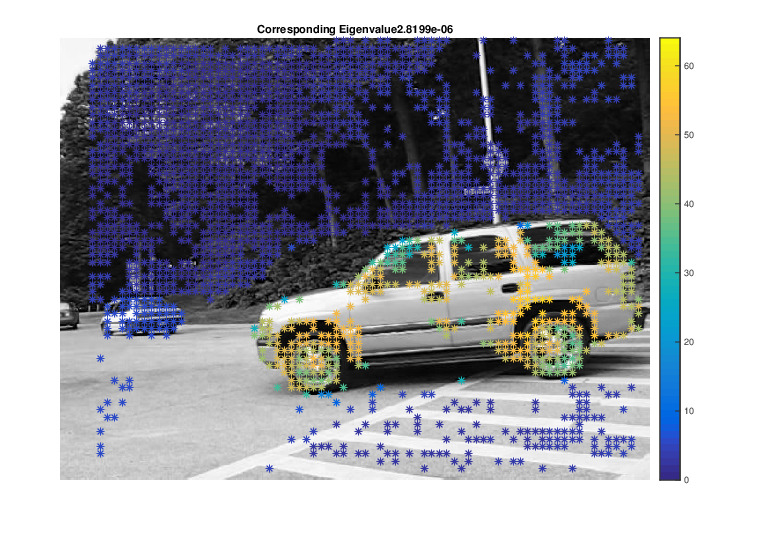
\includegraphics[width=0.48\linewidth] {derivation/eigenvectors/cars/ev_cf}
   \label{fig:cars_eigenvectors_laplacian_a}
}
\subfigure[Eigenvector Back-Car]{
   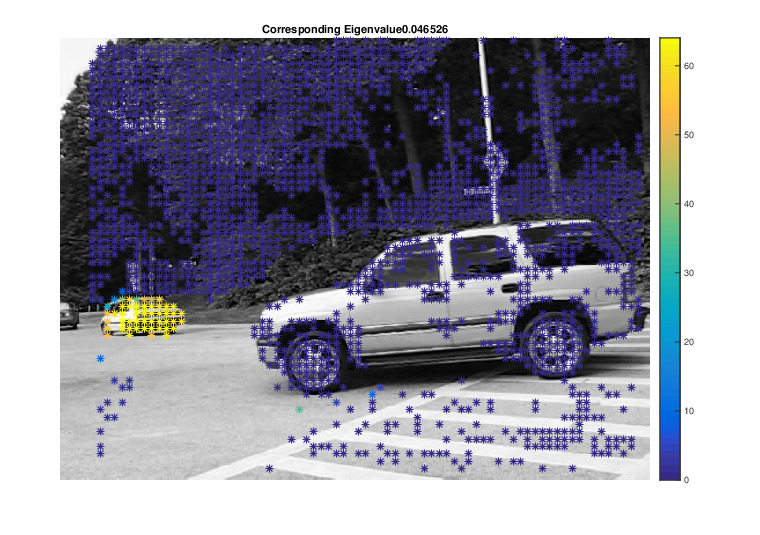
\includegraphics[width=0.48\linewidth] {derivation/eigenvectors/cars/ev_cb}
   \label{fig:cars_eigenvectors_laplacian_b}
}
\end{center}
\caption[Eigenvectors of the Laplacian]{Visualizing the contribution of two significant eigenvectors of the Laplacian of the affinity matrix that belong to the \textit{cars} dataset.}
\label{fig:cars_eigenvectors_laplacian}
\end{figure}

\begin{figure}[H]
\begin{center}
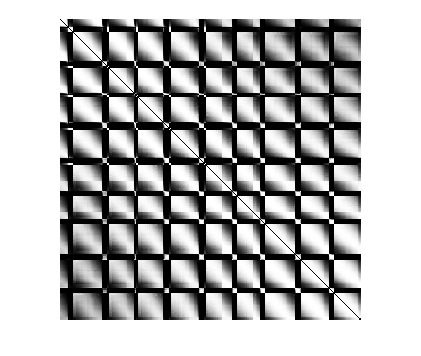
\includegraphics[width=0.7\linewidth] {derivation/eigenvectors/cars/w_mat}

\end{center}
\caption[Affinity Matrix W]{Visualization of the affinity matrix $W$ that belongs to the \textit{cars} dataset.}
\label{fig:cars_affinity_mat_sub}
\end{figure}
To obtain a simple segementation, we could run k-means on the first $k$ eigenvectors, that belong to the smallest k-eigenvalues. This approach yields a one-to-one mapping between cluster assignments and trajectory labels. However, the eigenvectors are often not piece-wise constant. Therefore, running k-means directly on the eigenvectors is not the best choice, since then the eigenvectors get approximated by multiple constant functions and thus the clustering yields an oversegementation. \\ \\
To address this issue we instead formulate a certain energy, containing a spacial regularity term that does not prefer spacial compact clusters. Moreover, it also takes edges in the eigenvectors into account. \\ \\
Let $v_i^A$ denote the $A-th$ component of the $i-th$ eigenvector in $V$ and $\bf{v}^A$ the vector composed of the $A-th$ components of the $m$ eigenvectors. Moreover, let $\mathcal{N}(A)$ denote the set of neighboring trajectories based on the spacial average distance. Then, we want to find the optimal cluster assignments $\pi^A \in {1, \dots, K}$ for a fixed, given number of clusters $K$, such that energy in equation $\ref{eq:min_cut_energy}$ gets minimized.	
\begin{equation}
\begin{aligned}
& E \left( \pi, K \right) = \sum_{A} \sum_{k=1}^K \delta_{\pi^A, k} \norm{\bf{v}^A - \mu_k}_{\lambda} + \nu \sum_A \sum_{B \in \mathcal{N}(A)} \frac{1- \delta_{\pi^A, \pi^B}}{\norm{\bf{v}^A - \bf{v}^B}} \\
& \text{where } \norm{\bf{v}^A - \bf{\mu}}_\lambda = \sum \frac{v_i^A -  \mu_i}{\lambda_i}
\end{aligned} 
\label{eq:min_cut_energy}
\end{equation}
The expression $\mu_k$ denotes the centroid of cluster $k$.

% TODO: explain the terms in the sum


\section{Minimum Cost Multicut Problem}
In this section we revisit the problem of finding an optimal graph partition by optimizing a certain energy, which is based on the work of $\cite{KB15b}$. Moreover, this derivation is also based on the concepts formulated in section $\ref{sec:graph_cut}$ on page $\pageref{sec:graph_cut}$. \\ \\
The minimum cost multicut problem is the problem of decomposing a graph $G = (V, E)$ into an optimal number of segments such that the overall cost in term of of edge weights $c_e$ is minimized. The node labeling problem can equivalently be formulated as a binary edge labeling problem
\begin{equation}
\begin{aligned}
& \min_{y \in \{0,1 \}^{|E|}} \sum_{e \in E} c_e y_e \\
& \text{subject to } y \in MC
\end{aligned}
\end{equation}
where $MC$ is the set of all characteristic functions of all multicuts. This corresponds to all $y \in \{0,1 \}^{|E|}$ that form a closed boundaries, representing a valid decomposition of the graph. \\ \\
A formal decomposition of these characteristic functions can be described as the follows:
\begin{equation}
	\forall C \in \text{cycles}(G) \forall e \in C: y_e \leq \sum_{e^{'} \in C \backslash \{e\}} y_{e^{'}}
\end{equation}
It was shown, that is is sufficient to consider all chordless cycles, i.e. all cycles in which each node is only connected to its successor and predecessor. To avoid trivial solutions, the edge weights are typically chosen to be negative for edges that should be cut and positive for those connection nodes that should be joined. \\ \\
Given the cut probabilities $p_e$ of an edge $e \in E$, the negative of the \textit{logit} function 
\begin{equation}
	\text{logit}\left( p_e \right) = \log \left( \frac{p_e}{1 - p_e} \right)
	\label{eq:logit_function}
\end{equation}
provides such a behavior. A plot if the negative logit function defined as in $\ref{eq:logit_function}$ is shown in figure $\ref{fig:negative_logit_function}$.
\begin{figure}
\centering
\begin{tikzpicture}[trim axis left]
\begin{axis}[
  axis x line=center,
  axis y line=center,
  grid=both,
  xtick={-2,-1,...,1,2},
  ytick={-2,-1,...,1,2},
  xlabel={$x$},
  ylabel={$-\text{logit}\left( x \right)$},
  xlabel style={below right},
  ylabel style={above left},
  no markers,
  xmin=-0.5,
  xmax=1.5,
  ymin=-1.5,
  ymax=1.5]
\addplot +[thick, domain=0:1] {-log10(x/(1-x)};
\end{axis}
\end{tikzpicture}
\caption[Logit Function Plot]{A plot of the negative logit function applied on the domain [0,1].}
\label{fig:negative_logit_function}
\end{figure}
If $p_e < 0.5$ then $\text{logit}\left( p_e \right) > 0$ and thus the according edge cost $c_e$ is positive and therefore the edge $e$ is expensive to be cut out from the graph. Conversely, in case that $p_e > 0.5$ the negative logit function of $p_e$ is smaller than zero and thus it is beneficial to cut e. \\ \\
For computing pseudo-probabilities, we use the inverse of the logit function, the so called logistic function
\begin{equation}
	f(z) = \frac{1}{1 + \exp \left( -z \right)}.
	\label{eq:logistic_function}
\end{equation}
The input values we put into the function from equation $\ref{eq:logistic_function}$ are computed by the transformed trajectory distances $d$:
\begin{equation}
	z \equiv z(d) = \beta_0 + \beta_1 d
\end{equation}
The prior probability of cutting two trajectories is defined by the intercept value $\beta_0$. Assuming we learned $\beta_0$ for a certain prior cut probability $p$ and are given a new prior cut probability $\tilde{p}$, we can adapt the value $z$ by
\begin{equation}
	z = \beta_0 - \log \left( \frac{p}{1-p} \right) + \log \left( \frac{\tilde{p}}{1-\tilde{p}} \right) + \beta_1 d.
\end{equation}
If the cut prior is increased, more edges will be cut and the number of resulting segments increases. Small cut priors results in an undersegmentation. \\ \\
In the following we define a measure for the trajectory distances. This distances makes use of the motion-, spatial- and color distance of the overlapping segments between two trajectories $A$ and $B$. Note that the definition of the motion distance is given by equation $\ref{eq:motion_distance}$ and the spatial distance is given by the definition stated in equation $\ref{eq:spatial_distance}$. For the color distance we compute the average color within the overlapping frames using the CieLab\footnote{The key property of the Cie Lab color space is that its values are uniformly spaced. This allows us to use the l2 norm in order to compute meaningful color differences.} color space. More precisely, the color distances $d_{color}$ is defined as the follows:

\begin{equation}
	d_{color}^{A,B} = \frac{1}{\omega - \alpha + 1} \sum_{k=\alpha}^\omega \norm{\text{ColorAt}(k, A(k)) - \text{ColorAt}(k, B(k))}_2
	\label{eq:color_dist}
\end{equation}
where $ColorAt(k, A(k))$ yields the CieLab color value in frame $k$ at the image location $A(k)$\footnote{Remember that $A(k)$ denotes the tracking position of trajectory $A$ in frame $k$}.
The final trajectory distance is computed by combining the described distance values as in equation $\ref{eq:sum_dist}$.
\begin{equation}
\begin{aligned}
z ( A, B ) = \max (\tilde{\beta_0} & + \beta_1 d_{motion}^{A,B} \\
& + \beta_2 d_{spatial}^{A,B} \\
& + \beta_3 d_{color}^{A,B},\\
\beta_0 & + \beta_1 d_{motion}^{A,B} )
\end{aligned}
\label{eq:sum_dist}
\end{equation}
If the sum of the spatial and the color distance is large in equation $\ref{eq:sum_dist}$ then only the motion distances are considered. This ensures that trajectories which are far apart but move similarly still end up in the same segment.

 
